\documentclass[a4paper,landscape,headrule,footrule,dvips]{foils}

%%
%%% macros for 2009 Semester 1 HG 803
%%%
\newcommand{\logo}{~}
\newcommand{\header}[3]{%
  \title{\vspace*{-2ex} \large HG3051  Corpus Linquistics
    \\[2ex] \Large  \emp{#2} \\ \emp{#3}}
  \author{\blu{Francis Bond}   \\ 
    \normalsize  \textbf{Division of Linguistics and Multilingual Studies}\\
    \normalsize  \url{http://www3.ntu.edu.sg/home/fcbond/}\\
    \normalsize  \texttt{bond@ieee.org}}
  \MyLogo{HG3051 (2018)}
  \renewcommand{\logo}{#2}
  \hypersetup{
    pdfinfo={
      Author={Francis Bond},
      Title={#1: #2},
      Subject={HG3051: Corpus Linguistics},
      Keywords={Corpus Linguistics},
      License={CC BY 4.0}
    }
  }
  \date{#1 \\ \url{https://github.com/bond-lab/Corpus-Linguistics}}
}

\usepackage{fontenc}
\usepackage{polyglossia}
\setmainlanguage{english}
\setmainfont{TeX Gyre Pagella}
%\setmainfont{Linux Libertine}
%\setmainfont{Charis SIL}
\newfontfamily{\ipafont}{Gentium}
\newcommand{\ipa}[1]{{\ipafont\selectfont #1}}
\usepackage{xeCJK}

\setCJKmainfont{Noto Sans CJK SC}
\setCJKsansfont{Noto Sans CJK SC}



\usepackage{xcolor}
\usepackage{graphicx}
\newcommand{\blu}[1]{\textcolor{blue}{#1}}
\newcommand{\grn}[1]{\textcolor{green}{#1}}
\newcommand{\hide}[1]{\textcolor{white}{#1}}
\newcommand{\emp}[1]{\textcolor{red}{#1}}
\newcommand{\txx}[1]{\textbf{\textcolor{blue}{#1}}}
\newcommand{\lex}[1]{\textbf{\mtcitestyle{#1}}}

\usepackage{pifont}
\renewcommand{\labelitemi}{\textcolor{violet}{\ding{227}}}
\renewcommand{\labelitemii}{\textcolor{purple}{\ding{226}}}

\newcommand{\subhead}[1]{\noindent\textbf{#1}\\[5mm]}

\newcommand{\Bad}{\emp{\raisebox{0.15ex}{\ensuremath{\mathbf{\otimes}}}}}
\newcommand{\bad}{*}

\newcommand{\com}[1]{\hfill \textnormal{(\emp{#1})}}%
\newcommand{\cxm}[1]{\hfill \textnormal{(\txx{#1})}}%
\newcommand{\cmm}[1]{\hfill \textnormal{(#1)}}%

\usepackage{relsize,xspace}
\newcommand{\into}{\ensuremath{\rightarrow}\xspace}
\newcommand{\ent}{\ensuremath{\Rightarrow}\xspace}
\newcommand{\nent}{\ensuremath{\not\Rightarrow}\xspace}
\newcommand{\tot}{\ensuremath{\leftrightarrow}\xspace}
\usepackage{url}
\newcommand{\lurl}[1]{\MyLogo{\url{#1}}}

\usepackage{mygb4e}
\let\eachwordone=\itshape
\newcommand{\lx}[1]{\textbf{\textit{#1}}}

%\usepackage{times}
%\usepackage{nttfoilhead}
\newcommand{\myslide}[1]{\foilhead[-25mm]{\raisebox{12mm}[0mm]{\emp{#1}}}\MyLogo{\logo}}
\newcommand{\myslider}[1]{\rotatefoilhead[-25mm]{\raisebox{12mm}[0mm]{\emp{#1}}}}
%\newcommand{\myslider}[1]{\rotatefoilhead{\raisebox{-8mm}{\emp{#1}}}}

\newcommand{\section}[1]{\myslide{}{\begin{center}\Huge \emp{#1}\end{center}}}



\usepackage[lyons,j,e,k]{mtg2e}
\renewcommand{\mtcitestyle}[1]{\textcolor{teal}{\textsl{#1}}}
%\renewcommand{\mtcitestyle}[1]{\textsl{#1}}
\newcommand{\chn}{\mtciteform}
\newcommand{\cmn}{\mtciteform}
\newcommand{\iz}[1]{\textup{\texttt{\textcolor{blue}{\textbf{#1}}}}}
\newcommand{\rel}[1]{\textsc{\color{blue}{#1}}}
\newcommand{\wn}[3]{\lex{#1}\ensuremath{_{#2:#3}}}
\newcommand{\con}[1]{\textsc{#1}}
\newcommand{\gm}{\textsc}
\usepackage[normalem]{ulem}
\newcommand{\ul}{\uline}
\newcommand{\ull}{\uuline}
\newcommand{\wl}{\uwave}
\newcommand{\vs}{\ensuremath{\Leftrightarrow}~}
\usepackage[hidelinks]{hyperref}
\hypersetup{
     colorlinks,
     linkcolor={blue!50!black},
     citecolor={red!50!black},
     urlcolor={blue!80!black}
}
%%%
%%% Bibliography
%%%
\usepackage{natbib}
%\usepackage{url}
\usepackage{bibentry}
%%% From Tim
\newcommand{\WMngram}[1][]{$n$-gram#1\xspace}
\newcommand{\infers}{$\rightarrow$\xspace}

\usepackage{bibentry}
\renewcommand{\cite}{\bibentry}

\header{Lecture 10}{Corpora and Language Engineering}{}

\usepackage{pst-node}
\newcommand{\sa}[2]{\rnode{c#1}{\iz{#2}}}%\nodebox{c#1}}

%\usepackage{hieroglf}
\usepackage{wasysym}
%\newcommand{\grn}[1]{\textcolor{PineGreen}{#1}}
\newcommand{\ont}[1]{\textcolor{blue}{#1}}
\newcommand{\jcy}[1]{\textcolor{orange}{#1}}
\newcommand{\lxd}[1]{\textcolor{brown}{#1}}


\newcommand{\psp}[1]{\textcolor{purple}{#1}}
\newcommand{\dtr}[1]{\textcolor{blue}{#1}}
\newcommand{\nam}[1]{\textcolor{blue}{#1}}
\newcommand{\idm}[1]{\textcolor{brown}{#1}}
\newcommand{\gen}[1]{\textcolor{orange}{#1}}
\newcommand{\exl}[1]{\textcolor{orange}{#1}}
\newcommand{\trg}[1]{\textcolor{red}{#1}}


\newcommand{\hinoki}{\grn{Hinoki}\xspace}
\newcommand{\lexeed}{\lxd{Lexeed}\xspace}
\newcommand{\jacy}{\jcy{JACY}\xspace}
\newcommand{\onto}{\ont{Ontology}\xspace}
%\newcommand{\itsdb}{\textsf{[incr tsdb()]}\xspace}
\newcommand{\GT}{Goi-Taikei\xspace}


\begin{document}
\begin{CJK}{UTF8}{min}
\bibliographystyle{apalike}
\nobibliography{abb,mtg,nlp,ling}
\maketitle


\myslide{Overview}

\begin{itemize} 
\item Revision of Contrastive and Diachronic Studies
  \begin{itemize} 
  \item Contrastive Studies
  \item Diachronic Studies
  \end{itemize}
\item Corpora and Language Engineering
  \begin{itemize}
  \item Language as a Statistical Model
  \item NLP and the Empirical Revolution
    \begin{itemize}
    \item Speech Recognition and Segmentation
    \item POS tagging, Word Sense Disambiguation and Parsing
    \item Machine Translation
    \end{itemize}
  \item The Empirical Revolution and Linguistics
  \end{itemize}
\end{itemize}
%%% 
%%% this changes each year, so keep separate
%%%
\include{schedule}

%%
%%% FIXME: Summarize
%%%

\myslide{Contrastive linguistics}

\begin{itemize}
\item  a linguistic approach that seeks to describe the differences and similarities between a pair of languages
\item Some of the many applications:
  \begin{itemize}
  \item to avoid interference errors in foreign-language learning
  \item to assist interlingual transfer in the process of translating texts from one language into another
  \item to find lexical equivalents in the process of compiling bilingual dictionaries, as illustrated
  \end{itemize}
\item generalized to the differential description of one or more varieties within a language, such as styles (contrastive rhetoric), dialects, registers or terminologies of technical genres
\end{itemize}


\myslide{Three Common Approaches}

\begin{itemize}
\item Look at examples in a \blu{translation lexicon}
  \begin{itemize}
  \item well aligned sample
  \item[x] no frequency information
  \end{itemize}
\item Look at examples in  \blu{comparable corpora}
  \begin{itemize}
  \item good for getting general trends
  \item[x] hard to measure \textbf{comparability}
  \end{itemize}
\item Look at examples in  \blu{aligned corpora}
  \begin{itemize}
  \item can get numbers at a very detailed level
  \item[x] translated text differs from monolingual text
  \item[x] translations can be very free
  \end{itemize}
\end{itemize}


\myslide{Three Studies}

\begin{itemize}
\item A Corpus based Comparison of Satellites in Chinese and English
  \begin{itemize}
  \item Comparable corpora used to compare verb+satellites
  \item General trends clear, but few conclusions
  \item Not clear how parallel the constructions are.
  \end{itemize}
\item Contrastive connectors in English and Chinese
  \begin{itemize}
  \item Parallel Corpora used to study  \textit{however} and its Chinese counterparts
    \begin{itemize}
    \item the HLM parallel corpus
    \item the Babel English-Chinese Parallel Corpus
    \end{itemize}
  \item a deep analysis of a small number of examples
  \item very different results for the different samples
  \end{itemize}
\newpage
\item A Parallel Corpus-based Study of Translational Chinese
\begin{itemize}
\item Compared English Text (EST), Original Chinese Text (OCT),
  Translated Chinese Text (TCT)
\item Translational Chinese has the following features
  \begin{itemize}
  \item TCT uses fewer monosyllabic words than OCT does
  \item compared with OCT, TCT uses more function words
  \item TCT can change or expand the compositionality of some words or morphemes in
    Chinese.
\end{itemize}
\item TCT use more types and longer segments than OCT. This does not
  support the hypothesis of lexical and syntactic simplification in translation.
\end{itemize}
\end{itemize}

\myslide{Historical Linguistics}
\begin{itemize}
\item All Historical linguistics is corpus linguistics: we can not ask
  Old English speakers for grammatical judgments
\item The texts of a historical period or a dead language form a closed corpus 
  \begin{itemize}  \item  can only be extended by the (re-)discovery of previously unknown texts
  \end{itemize}
\item Comparable corpora sampled over different times have made it
  possible to quantitatively study language change %over time
\begin{itemize}
\item \blu{Helsinki Corpus of English Texts: Diachronic and Dialectal}
  \\ 1.6 million words of British English from 750 to 1700 (Old/Middle/Modern)
\item \blu{Corpus of Historical American English} has been created
\\  400 million words of text of American English from 1810 to 2009. 
\item \url{http://ngrams.googlelabs.com/}
\end{itemize}
\end{itemize}


\myslide{The \lex{by}-agent in English}

\begin{itemize}
\item  Peitsara (1993) used four subperiods from the Helsinki corpus to calculate the frequencies of different prepositions introducing agent phrases
  \begin{itemize}
  \item In late Middle English (\eng{c.} 1350) \eng{of} and
    \eng{by} were in roughly equal distribution (10.6:9)
  \item By the fifteenth century \eng{by} was three times more
    common than \eng{of}
  \item By 1640 \eng{by} was eight times as common
  \end{itemize}
\item There was marked influence of text type: statutes and official
  documents were much more likely to use \eng{by}
  \begin{itemize}
  \item This is probably due to bilingual influence from French
  \end{itemize}
\end{itemize}


Peitsara, K. (1993) "On the development of the by-agent in English", in \textit{Early English in the Computer Age}. Rissanen, Kytö and Palander-Collin eds, 1993 pp 217-33, Berlin, Mouton de Gruyter. 

\myslide{The case of it’s and ‘tis}
Peitsara, K. (2004) ``Variants of contraction: The case of it’s and ‘tis'' \textit{ICAME} \textbf{28} pp 77-94

\begin{itemize}
\item two contracted forms of \eng{it is}
  \begin{itemize}
  \item \eng{'tis} (\eng{tys, ‘t is, t is, t‘ is})
  \item \eng{it's} 
  \end{itemize}
\item Contractions are more often used in speech than text: hard to study historically
\item Big shift to \eng{it's} between 1800 and 1850
\item Part of a general trend from proclisis (initial) to enclisis (embedded)
\end{itemize}

\myslide{Issues with Historical Linguistics}
\MyLogo{}
Rissanen (1989) identifies three problems  with using historical corpora
\begin{itemize}
\item The \blu{philologist's dilemma} ---the danger that the use of a corpus and a computer may supplant the in-depth knowledge of language history which is to be gained from the study of original texts in their context
\item  The \blu{God's truth fallacy} --- the danger that a corpus may be used to provide representative conclusions about the entire language period, without understanding its limitations in the terms of which genres it covers.
\item The \blu{mystery of vanishing reliability} --- the more variables which are used in sampling and coding the corpus (periods, genres, age, gender etc) the harder it is to represent each one fully and achieve statistical reliability. The most effective way of solving this problem is to build larger corpora of course
\end{itemize}



\section{Corpora and Language Engineering}


%%%
%%% Evaluation and the Empirical Revolution
%%%
\myslide{Testing and Training}

\begin{itemize}
\item Language Engineering use Corpora in two important ways:
  \begin{itemize}
  \item Testing
    \begin{itemize}
    \item Create a \blu{reference set} or \blu{gold standard}
    \item Test how well a system can produce these results
    \end{itemize}
  \item Training
   \begin{itemize}
    \item Create a collection of \blu{labeled examples}
    \item Use these to learn features to classify new examples with
      one of the labels
    \end{itemize}

  \item Models are implicit in the corpus, rather than written by hand
  \item Even which features are useful can be learned
  \item Annotation becomes the bottleneck
  \end{itemize}
\end{itemize}

\myslide{Classical NLP}

\begin{itemize}
\item In classical NLP, researchers developed rules based on their own
  intuition and tested them on small test suites they themselves created
\item Such systems proved hard to scale to large problems
\item In particular, many systems required a large amount of knowledge:
  \begin{itemize}
  \item words given their pronunciation
  \item words classified by part of speech
  \item words classified by semantic class
  \item predicates classified by argument structure
  \end{itemize}
Creating and maintaining these is expensive and difficult:
\\ \blu{the resource bottleneck}
\end{itemize}

\myslide{The breakthrough in speech recognition}

\begin{itemize}
\item There was a great breakthrough in speech recognition
  \begin{itemize}
  \item transcribe corpora, align the text and speech,
    and then learn pronunciations from the aligned data
    \begin{itemize}
    \item Easier to do than writing IPA for each word
    \item More natural data --- includes performance changes
    \item Easy to go back and look at more features
    \end{itemize}
  \item share data (prompted by funding agencies)
  \item share test data (with an agreed on metric)
  \end{itemize}
\item System quality increased very quickly
\item Shallow (non-cognitive) approaches began to dominate
%\item Performance plateaued well below human performance
\end{itemize}


\myslide{Word Error Rate in Speech Recognition}

\begin{itemize}
\item The first successful wide spread testing:
  \begin{itemize}
  \item Compare your output to a reference
  \item Calculate the number of substitutions, deletions and insertions to make them match
(Minimum edit distance)
  \item Normalize by dividing by the length of the reference\\[2ex]
    {\Large
    $\begin{array}{lcr}
      WER = \frac{S+D+I}{N}
    \end{array}$
}
  \end{itemize}

\item 
  \begin{tabular}[t]{llllllllll}
    Reference: & I &want &to &recognize&  & &speech & today \\
    System:    & I &want &   &wreck    &a &nice &peach & today\\
    Eval:      &   &     & D   & S       & I & I & S \\
  \end{tabular}
\item $WER=\frac{2+1+2}{6}=0.8$

\end{itemize}


\myslide{Some properties of WER}

\begin{itemize}
\item Correlates well with the task
\item Reducing WER is always a good thing
\item A WER of 0 implies perfect results
  \\ (assuming the reference is correct)
\item $WER < 0.05$ considered the threshold to be useful
\item Competitions were held to see who could get the lowest WER
  \begin{itemize}
  \item Speech Recognition had 10 years of rapid improvement
  \item It has slowed down now
  \end{itemize}
\end{itemize}

\myslide{How good are the systems?}

  \begin{tabular}{lrrr}
    Task & Vocab & WER (\%) & WER  (\%) adapted \\ \hline
    Digits & 11 & 0.4 & 0.2 \\
    Dialogue (travel) & 21,000 & 10.9 & --- \\
    Dictation (WSJ) & 5,000 & 3.9 & 3.0 \\
    Dictation (WSJ) & 20,000 & 10.0 & 8.6 \\
    Dialogue (noisy, army) & 3,000 & 42.2 & 31.0 \\
    Phone Conversations & 4,000 & 41.9 & 31.0 \\
  \end{tabular}

Speaker adapted systems have a lower WER.

(2014) New Deep-learning based approaches may have reduced errors by as much as 30\%.

Another nice feature of training on data --- new algorithms arise and
can be exploited

\myslide{WER Task}
Calculate the WER for the following pairs:

\begin{exe}
\ex 
  \begin{xlist}
    \ex HYP:  \eng{What alright day}
    \ex REF:  \eng{What a bright day}
  \end{xlist}
\medskip
\ex 
  \begin{xlist}
    \ex HYP:  \eng{uno fantas grandes de limon}
    \ex REF:  \eng{dos fantas grandes de limon}
  \end{xlist}
\medskip
\ex 
  \begin{xlist}
    \ex HYP:  \eng{excuse me while I kiss this guy}
    \ex REF:  \eng{'scuse me while I kiss the sky}
  \end{xlist}
\medskip
\ex
 \begin{xlist}
    \ex HYP:  \eng{Baby come back, you can play Monopoly}
    \ex REF:  \eng{Baby come back, you can blame it all on me}
  \end{xlist}
\end{exe}


\myslide{The need for automatic testing}
\MyLogo{}
\begin{itemize}
\item As systems get bigger, behavior is harder to predict
\item Looking at system output one sentence at a time is slow

\item Can we automate testing?
  \begin{enumerate}
  \item Create a gold standard or reference (the \blu{right} answer)
  \item Compare your result to the reference
  \item Measure the error
  \item Attempt to minimize it \blu{globally} (over a large test set)
    \begin{itemize}
    \item \textit{the plural of anecdote is not data}
    \item intuition tends to miss many examples of use
    \end{itemize}
  \end{enumerate} 

\end{itemize}

\myslide{The Empirical approach}

\begin{enumerate}
\item Develop an algorithm and gather examples/rules from \blu{training data}
\item Optimize any parameters on \blu{development data}
  \begin{itemize}
  \item Normally about 10\% of the training data
  \end{itemize}
\item Test on held-out, unseen \blu{test data}
\end{enumerate}

This gives a fair estimate of how good the algorithm is 
\\ --- if the test criteria are appropriate.


\myslide{Empirical vs Rational NLP}
  \begin{itemize}
  \item The 1990s went through an empirical revolution
  \item Funding agencies sponsored competitions
    \begin{itemize}
    \item TREC: Text REtrieval Conference
    \item MUC: Message Understanding Conference
    \item DARPA Machine Translation Competitions
    \end{itemize}
  \item Data to test with became more available
  \item Reviewers demanded evaluation in papers
  \item A lot of research on evaluation methods
  \end{itemize}


\myslide{Machine Translation Evaluation}

\begin{itemize}
\item Evaluating MT output is non-trivial
  \begin{itemize}
  \item There may be multiple correct answers 
    \\ 泳ぐ\,の\,が\ 好き\,だ \jpn{oyogu-no-ga suki-da}
    \begin{itemize}
    \item \eng{I like to swim}
    \item \eng{I like swimming}
    \item \eng{Swimming turns me on}
    \end{itemize}
  \end{itemize}
\item Hand evaluation requires a bilingual evaluator - expensive
\item Automatic evaluation can be done by comparing results (in a held
  out test  set) to a set of reference translations
  \begin{itemize}
  \item The most common metric is BLEU 
  \item Other scores are: Word Error Rate; METEOR
  \end{itemize}
\end{itemize}



\myslide{MT Evaluation: Fluency and Adequacy}
\begin{itemize}
\item \txx{Fluency:} How do you judge the fluency of this translation?
\begin{itemize}\item 5 = Flawless English 
\item 4 = Good English 
\item 3 = Non-native English 
\item 2 = Disfluent English 
\item 1 = Incomprehensible 
\end{itemize}
\item \txx{Adequacy:} How much of the meaning expressed in the reference
  translation is also expressed in the hypothesis translation? 
\begin{itemize} 
\item 5 = All  
\item 4 = Most  
\item 3 = Much  
\item 2 = Little  
\item 1 = None 
\end{itemize}
\end{itemize}


\myslide{MT Evaluation: The BLEU score}
\begin{itemize}
\item BLEU score compares n-grams (normally up to 4) with those in the
  reference translation(s) (with a brevity penalty)

\[BLEU \approx\sum_{i=1}^{n} \frac{\textnormal{n-grams in sentence and reference}}{|\textnormal{n-grams}|}\]

\item 0.3--0.5 typical; 0.6+ approaches human
\item Only really meaningful summed over a test set
  \begin{itemize}
  \item individual sentences are too short
  \end{itemize}
\end{itemize}




\myslide{An example of BLEU}
  \hspace{-3em}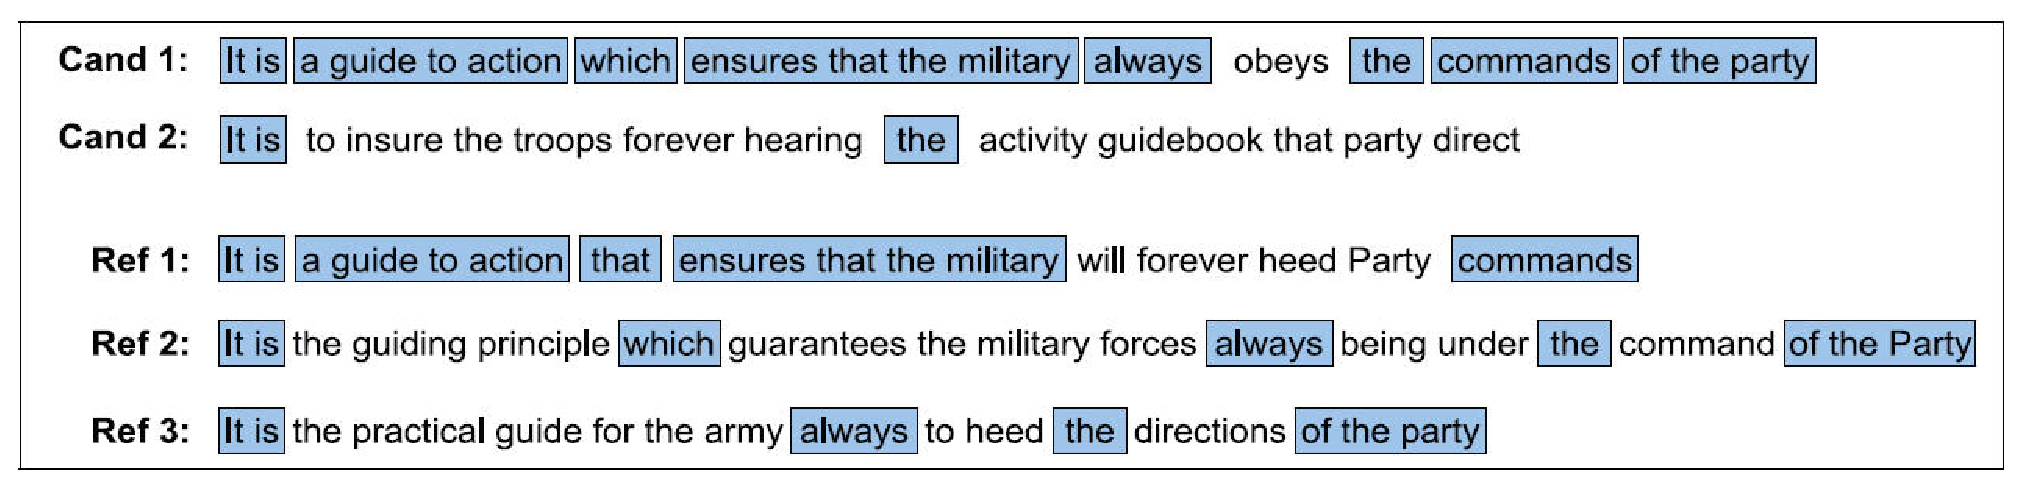
\includegraphics[width=1.1\textwidth]{include/25.31.jpg.eps}

  \begin{center}
    Intuition for BLEU (from Jurafsky and Martin Fig 25.31)
  \end{center}

\myslide{An Example of Variation}

\begin{enumerate}
\item \textit{Early and frequent releases are a critical part of the Linux development model}
  \begin{enumerate}
  \item 早期 かつ 頻繁 な 公開 は 、 リナックス の 開発 モデル の 重要 な 部分 で ある 。% grid
  \item 早く 、 そして 頻繁 に 公表 する こと は リナックス の 発展 モデル の 重要 な 一部 で ある 。 % nakatsuji
  \item 早く 、 そして 頻繁 な リリース は 、 Linux 開発 モデル にとって は 重要 な 部分 で ある 。 % yoshimura
  \end{enumerate}
\end{enumerate}

\hspace{-20mm}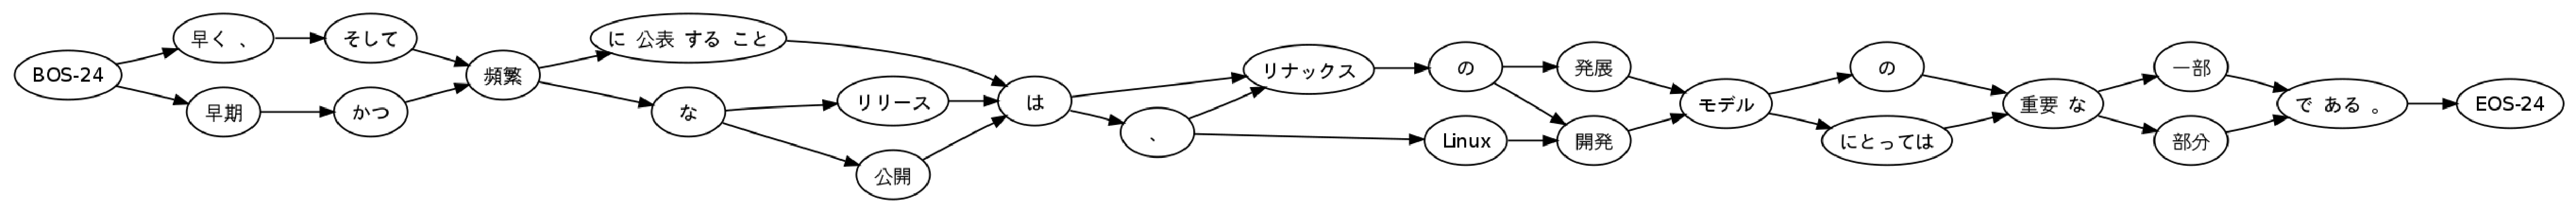
\includegraphics[width=1.2\textwidth]{include/lattice-24.eps}

\myslide{1-grams (56)}
\begin{small}
\begin{verbatim}
な<>5 
の<>4 
は<>4 
で<>3 
モデル<>3 
ある<>3 
頻繁<>3 
EOS<>3 
BOS<>3 
重要<>3 
早く<>2 
部分<>2 
リナックス<>2 
開発<>2 
そして<>2 
こと<>1 
\end{verbatim}
\end{small}


\myslide{2-grams (55)}
\begin{small}
\begin{verbatim}
で<>ある<>3 3 3 
重要<>な<>3 3 5 
ある<>EOS<>3 3 3 
な<>部分<>2 5 2 
頻繁<>な<>2 3 5 
は<>リナックス<>2 4 2 
早く<>そして<>2 2 2 
開発<>モデル<>2 2 3 
EOS<>BOS<>2 2 2 
BOS<>早く<>2 3 2 
リナックス<>の<>2 2 4 
モデル<>の<>2 3 4 
の<>重要<>2 4 3 
そして<>頻繁<>2 2 3 
部分<>で<>2 2 3 
は<>重要<>1 4 3 
は<>Linux<>1 4 1 
\end{verbatim}
\end{small}

\myslide{3-grams (54)}
\begin{small}
\begin{verbatim}
で<>ある<>EOS<>3 3 3 3 3 3 3 
ある<>EOS<>BOS<>2 2 2 2 2 2 2 
は<>リナックス<>の<>2 4 2 4 2 2 2 
部分<>で<>ある<>2 2 3 3 2 2 3 
重要<>な<>部分<>2 3 5 2 3 2 2 
EOS<>BOS<>早く<>2 2 2 2 2 2 2 
早く<>そして<>頻繁<>2 2 2 3 2 2 2 
の<>重要<>な<>2 4 3 5 2 2 3 
BOS<>早く<>そして<>2 3 2 2 2 2 2 
な<>部分<>で<>2 5 2 3 2 3 2 
モデル<>の<>重要<>2 3 4 3 2 2 2 
こと<>は<>リナックス<>1 1 4 2 1 1 2 
は<>重要<>な<>1 4 3 5 1 1 3 
頻繁<>な<>公開<>1 3 5 1 2 1 1 
そして<>頻繁<>に<>1 2 3 1 2 1 1 
\end{verbatim}
\end{small}

\myslide{4-grams}

\begin{itemize}
\item No four grams!
\end{itemize}

% \subhead{BLEU}

% Overlap between 

\myslide{BLEU pros and cons}
  \begin{itemize}
\item Good
  \begin{itemize}
  \item Easy to calculate (if you have reference translations)
  \item Correlates with human judgement to some extent
  \item Used in standard competitions
  \end{itemize}
\item Bad
  \begin{itemize}
  \item Doesn't deal well with variation
    \begin{itemize}
    \item Exact string match
    \item Near misses score zero: \eng{cat} $\ne$ \eng{cats}!
    \end{itemize}
  \item Biased toward n-gram models
    \begin{itemize}
    \item SMT systems optimize for BLEU
    \end{itemize}
  \end{itemize}
\end{itemize}




\myslide{Misleading Bleu Scores}
\begin{itemize}
\item 信号は赤でした。
  \begin{itemize}
  \item \blu{The \ul{light} was red.}
  \item The \ul{signal} was red. \com{0.35}
  \end{itemize}
\item  大丈夫です。
  \begin{itemize}
  \item \blu{\ul{I'm} all right.}
  \item \ul{I am} all right. \com{0.27}
  \end{itemize}
\item  空港から電話しています。
  \begin{itemize}
  \item \blu{\ul{I'm} \ul{calling} from the \ul{airport}.}
  \item \ul{I am} \ul{telephoning} from the \ul{airports}.\com{0.22}
  \end{itemize}
\end{itemize}


\myslide{How to improve the reliability?}

\begin{itemize}
\item Use more reference sentences
\item Use more translations per sentence
  \begin{itemize}
  \item Can be automatically created by paraphrasing
  \end{itemize}
\item Improve the metric: METEOR
  \begin{itemize}
  \item add stemmed words (partial score): \eng{cat} $\approx$ \eng{cats}!
  \item add WordNet matches (partial score): \eng{cat} $\approx$ \eng{feline}!
  \end{itemize}
\item Unfortunately this adds noise 
  \begin{itemize}
  \item Errors in stemming
  \item Uneven cover in WordNet
  \end{itemize}
\item Still better than BLEU (so far) --- but harder to calculate
\end{itemize}




\myslide{Problems with testing}


\begin{itemize}
\item {\large You get better at what you test}
\item If the metric is not the actual goal things go wrong
  \begin{itemize}
  \item  BLEU score originally correlated with human judgement
  \item As systems optimized for BLEU
  \item \ldots they lost the correlation
  \item You can  improve the metric, not the goal
  \end{itemize}
\item The solution is better metrics, but that is hard for MT
\item We need to test for similar meaning: a very hard problem
\end{itemize}


% \myslide{MRS Test Set (Functional)}
% \begin{itemize}
% \item Minimal Recursion Semantics Test Set (for English)
% \item En-(Ja, De, Fr, Gr, Es, Po, No, \ldots)
% \item 117 sentences
%   \begin{itemize}
%   \item 1 argument \\ 太郎 が 吠え た . \\ Abrams barked.
%   \item 1 argument inchoative \\ 窓 が 開い た . \\ The window opened.
%   \item 2 arguments \\ 太郎 が 次郎 を 追っ た . \\ Abrams chased Browne.
% \end{itemize}
% \end{itemize}

 \myslide{Variation in Translation (MRS Test set)}
\MyLogo{Translated by my students in Nara Women's University}

\begin{enumerate}
\item \textit{The dog to chase is barking.}
  \begin{enumerate}
  \item 追う べき 犬 が 吠え て いる .
  \item 追いかけよ う と する 犬 が 吠え て いる 。
  \item 追いかけ られ て 、 その 犬 は 吠え て いる 。 
  \end{enumerate}
\item \textit{The dog was chased by Browne.}
  \begin{enumerate}
  \item 犬 が ブラウン に 追わ れ た .
  \item その 犬 は ブラウン に 追いかけ られ た 。
  \item その 犬 は 、 ブラウン さん に 追いかけ られ た 。
  \end{enumerate}
\newpage
\item \textit{The dog chased by Browne barked.}
  \begin{enumerate}
  \item ブラウン に 追わ れ た 犬 が 吠え た .
  \item ブラウン に 追いかけ られ て いる 犬 が 吠え た 。
  \item ブラウン さん に 追いかけ られ た 犬 は 、 吠え た 。 
  \end{enumerate}
\item \textit{The dog is barking.}
  \begin{enumerate}
  \item 犬 が 吠え て いる .
  \item 犬 が 吠え て いる 。
  \item その 犬 は 吠え て いる 。 
  \end{enumerate}
\item \textit{The dog has barked.}
  \begin{enumerate}
  \item 犬 が 吠え た こと が ある .
  \item 犬 が 吠え た 。
  \item その 犬 は さっき から 吠え て いる 。 
  \end{enumerate}
\item \textit{The dog has been barking.}
  \begin{enumerate}
  \item 犬 が 吠え て い た .
  \item 犬 が ずっと 吠え て いる 。
  \item その 犬 は さっき から ずっと 吠え て いる 。 
  \end{enumerate}
\item \textit{The dog had been barking.}
  \begin{enumerate}
  \item 犬 が 吠え て い た .
  \item 犬 が ずっと 吠え て い た 。
  \item その 犬 は さっき まで ずっと 吠え て い た 。 
  \end{enumerate}
\item \textit{The dog will bark.}
  \begin{enumerate}
  \item 犬 が 吠える だろ う .
  \item その 犬 は 吠える だろ う 。
  \item その 犬 は 吠え そう で ある 。
  \end{enumerate}
\item \textit{The dog is going to bark.}
  \begin{enumerate}
  \item 犬 が 吠える ところ だ .
  \item 犬 が 吠えよ う と し て いる 。
  \item その 犬 は 今 に も 吠え そう だ 。 
  \end{enumerate}
\newpage
\item \textit{The dog could bark.}
  \begin{enumerate}
  \item 犬 が 吠え こと が できる .
  \item 犬 が 吠え られる .
  \item その 犬 は 吠える こと が でき た 。
  \item その 犬 は 吠える 可能 性 が ある 。 
  \end{enumerate}
\item \textit{The dog couldn't bark.}
  \begin{enumerate}
  \item 犬 が 吠える こと が でき ない .
  \item 犬 が 吠え られ ない .
  \item その 犬 は 吠える こと が でき なかっ た 。
  \item その 犬 が 吠える 可能 性 は ない 。 
  \end{enumerate}
\end{enumerate}




\myslide{Conclusion}
\begin{itemize}
\item A surprising amount of variation is possible in MT
  \\ so you need a lot of data for a reliable evaluation
\item This makes evaluation difficult
  \begin{itemize}
  \item If we know a correct answer, the problem is still not solved
  \end{itemize}
\item But evaluation is very important in NLP
  \begin{itemize}
  \item Use automatic evaluation
  \item Recognize the risks
  \end{itemize}
\end{itemize}


\myslide{Coverage and OOV}

\begin{itemize}
\item The resource bottleneck still exists in several forms
  \begin{itemize}
  \item We don't have corpora for all tasks in all languages
  \item In-domain training data much better than out-of-domain training data
  \item More out-of-domain data only helps a little
  \end{itemize}
\item For those we do there are still Out of Vocabulary items (OOV)
\item Distribution is domain dependent
\item The bottleneck has shifted from lexicons to corpora
\end{itemize}

\myslide{Domain dependence}
\MyLogo{Danile Gildea \textit{Corpus Variation and Parse Performance} EMNLP 01}

\begin{center}
  \begin{tabular}{ll|rr}
    Training Data & Test Set & Recall & Precision \\
    \hline
    WSJ & Brown &   80.3 & 81.0 \\
    Brown & Brown & 83.6 & 84.6 \\ 
    WSJ+Brown & Brown & 83.9 & 84.8 \\ 
    WSJ & WSJ & 86.1 & 86.6 \\
    WSJ+Brown & WSJ & 86.3 & 86.9 \\ 
  \end{tabular}
  \\[2ex] tested using similar test sets, 
  \\ training data roughly twice as large for WSJ, 
  \\ precision/recall measured with labeled parse constituents
  \\ Brown is non-homogeneous, WSJ is homogeneous
\end{center}

\begin{itemize}
\item Models over-fit to their training data
\item Language use is slightly different in different genres
\end{itemize}

\myslide{Training from Corpora: POS tagging}
\MyLogo{}
\begin{itemize}
\item Learn rules automatically from tagged text
  \begin{itemize}
  \item Many learning methods
  \item Current popular learner is MIRA, before then CRF, before then SVM, \ldots
  \item Algorithms and CPU speeds are improving
  \end{itemize}
\item 96\%+ accuracy using these features (probability based)
  \begin{itemize}
  \item Previous $n$ words, (succeeding $n$ words)
  \item Previous $n$ tags
  \item Combinations of words and tags
  \item Word Shape
\end{itemize}
\item Learning methods relatively language independent 
  \\ but corpora and standards must exist
%\item Japanese examples: ChaSen (茶筌), MeCab (和布蕪)
\end{itemize}

\myslide{Out of Vocabulary (OOV) words}
\MyLogo{}
\begin{itemize}
\item Unknown words are a big problem
  \begin{itemize}
  \item Completely unknown words (not in lexicon)
  \item Unknown uses of known words (derivation or lexicon gaps)
  \end{itemize}
\item Big, accurate lexicons are most useful!
\item Otherwise guess from \blu{word shape} (and context)
  \begin{itemize}
  \item lowercase \into common noun
  \item uppercase \into Proper noun
  \item ends in \textit{-ly} \into adverb
  \item ends in \textit{-ing} and has vowel \into verb
  \item character type (Chinese character, alphabet, number, kana, \ldots)
  \end{itemize}
\item You can learn these features (look at last $n$ letters, \ldots)
\end{itemize}

\myslide{Some issues}

\begin{itemize}
\item You get best results for things you have seen before
  \begin{itemize}
  \item so if you are trying to extract knowledge, you reinforce what
    you already know
  \item there are many underlying assumptions to text mining
    \begin{itemize}
    \item you can tokenize
    \item your sample is representative
    \end{itemize}
  \item in theory, data-driven is language agnostic
    \begin{itemize}
    \item but tools are developed on major languages
    \item our models work better for analytic languages
    \item subversive text is likely to be harder to find
    \end{itemize}

  \end{itemize}
\end{itemize}


\myslide{Conclusion}

\begin{itemize}
\item Testing on corpora objectively reveals system properties
\item Training learns features humans don't predict
  \begin{itemize}
  \item we are bad at simple frequency counts
  \end{itemize}
\item Training and Test have to be separate
\item The closer the training is to the test, the better the result
\item The general conclusion: \blu{more data is better data}
\end{itemize}


%%
%% Future
%%
\clearpage
\end{CJK}
\end{document}

% Local Variables: 
% TeX-view-style: (("." "xdvi-ja %d -paper a4r -s 7"))
% LaTeX-section-list:  (("myslide" 1))
% TeX-master: t
% End:
